
\chapter{Physical Foundations of Multiphase flows}

\section{Introduction}
 
Three main forces are considered in the regime of multiphase flows: Pressure, Viscous and Surface Tension forces. \\
\noindent
In the following sections we discuss the calculations of Surface tension forces. \\
\noindent
To calculate the surface tension force, we will need to calculate the interface curvature of different phases.

\section{Interface Tracking Techniques}

In the case of immiscible fluids, each corresponding to a differenct 'color', c, interface tracking can be achieved by simulating the advection of the color function. \cite{Morris}

\begin{equation}
\frac{\partial c}{\partial t} + \mathbf{v}.\nabla c = 0 
\end{equation}

The color function may be evolved in a Lagrangian fashion by assigning it as a physical property to 'particles', which are then advected through the computational domain. In genral, this may be achieved using particles on the interface alone(surface-marker methods) or by employing particles which fill the entire computational domain(volume-marker methods). Surface markers have been used extensively to track the location of interface with high accuracy. This approach may be exploited by fully Lagrangian Techniques like SPH. With SPH, each extra phase is modelled simply by introducing an extra species of a particle of different color property.

\section{The Continuum Surface Force Method}

The Continuum surface force(CSF) method \cite{Brackbill} permits numerical simulation of surface tension without placing restrictions upon the flow geometry. The CSF approach models process localized to a fluid interface by applying them to fluid elements in the transition region of the interface. Interfacial phenomena, such as surface tension and phase change, are translated into volume processes having a net effect that emulates the desired physics.
In the CSF model, surface tension is translated into a force per unti volume $\mathbf{F_s}$, by

\begin{equation}
 \mathbf{F_s} = \mathbf{f_s} \delta_s
\end{equation}

\noindent
where $\delta_s$ is a normalized surface delta function, which peaks at the interface and $\mathbf{f_s}$ is the force per unit area given by

\begin{equation}
 \mathbf{f_s} = \sigma \kappa \mathbf{\hat{n}} + \nabla_s \sigma
 \label{forceperarea}
\end{equation}

\noindent
where $\sigma$ is the surface tension coefficient, $\mathbf{\hat{n}}$ is the unit normal to the interface, $\kappa$ is the curvature to the interface and $\nabla_s$ is the surface gradient. The second term in \ref{forceperarea} acts tangentially to the interface, forcing fluid from regions of low surface tension to higher surface tension. In this work surface tension is assumed constant throughout the fluid and hence that part is neglected. The first term in \ref{forceperarea} acts normal to the interface corresponding to the net surface tension force due to the local curvature. This force acts to smooth regions of high curvature, in an attempt to reduce the total surface energy.
The normal in \ref{forceperarea} can be obtained using

\begin{equation}
 \mathbf{n} = \frac{\nabla c}{[c]}
\end{equation}

\noindent
where c is the color function identifying each fluid in the simultion and [c] is the jump in c across the interface. The curvature can be calculated as
\begin{equation}
 \kappa = \nabla . \mathbf{\hat{n}}
\end{equation}

\noindent
There are many possible choices for $\delta_s$ however, it should be normalized such that its integral through the boundary is one. This is necessary for the correct physics of the interface to be recovered as the resolution is increased. The funciton should also be non-zero only in those fluid elements that correspond to the transition regions in the numerical method. The surface delta function employed in this work is

\begin{equation}
 \delta_s = \left| \mathbf{n} \right |
\end{equation}


\chapter{SPH formulations}

Using SPH, the fluid is represented by particles, generally of fixed mass, which follow the fluid motion according to their governing differential equations. These governing equations become expressions for interparticle forces and fluxes when written in SPH form. Using the standard approach of SPH, the particles move with the local fluid velocity carrying a mass m. Each particle has it's own velocity $\mathbf{v}$ and other fluid quantities specific to the given problem. 

\section{Density}

Density is evaluated for every particle at the beginning of the time step using the following equation called as Summation Density. 

\begin{equation}
 \rho_a = \sum_b m_b W_{ab}
\end{equation}

\noindent
where $W_{ab}$ denotes

\begin{equation}
 W_{ab} = W(\mathbf{r_{ab}}, h)
\end{equation}

\noindent
and

\begin{equation}
 \mathbf{r_{ab}} = \mathbf{r_a} - \mathbf{r_b}
\end{equation}
\noindent
where $\mathbf{r_a}$ denotes the position of particle a. The kernel typically takes the form

\begin{equation}
 W(\mathbf{r_{ab}}, h)= \frac{1}{h^N} f\left( \frac{\left|\mathbf{r_{ab}} \right|}{h}\right)
\end{equation}
\noindent
where N is the number of dimensions and the function f is typically either a Gaussian or a spline approximating a Gaussian. The smoothing length is generally between 1-1.5 times the shortes particle separation. 

\section{Equation of State}
In SPH, pressure is an explicit function of local fluid density and a quasi-incompressible equation of state is used. For this work, the isothermal EOS as follows is used.

\begin{equation}
 p_a = c_s^2 (\rho_a - \rho_0)
\end{equation}

\noindent
where $\rho_0$ is the reference density of the fluid and $c_s$ is the artificial speed of sound. Subtracting the reference density was found to lead to more accurate simulations. The reason for this is that subtracting the reference density removes a zeroth-order term associated with conservative forms of SPH pressure gradients. The speed of sound is chosen to be generally 10 times the maximum velocity of the particles. 

\section{Forces}

The forces in the simulations are divided into three parts:

\begin{itemize}
 \item Pressure forces
 \item Viscous forces
 \item Surface Tension forces
\end{itemize}

\subsection{Pressure Forces}

The pressure forces are caused due to pressure gradients. The SPH expression used to approximate the pressure gradient term in this work is:

\begin{equation}
 -\left( \frac{1}{\rho} \nabla p\right)_a = -\sum_b m_b \left( \frac{p_a + p_b}{\rho_a \rho_b}\right) \nabla_a W_{ab}
\end{equation}
\noindent
where $p_a$ is the pressure at particle a and $\nabla_a$ denotes the gradient with respect to the co-ordinates of particle a. This form of pressure gradient conserves momentum exactly, since forces acting between individual particles are antisymmetric.

\subsection{Viscous Forces}

Viscous forces were calculated using a formulation recently applied to low Reynolds Number flow. \cite{viscous} The SPH momentum equation may be written as \cite{viscous}:

\begin{equation}
 \left(\frac{d\mathbf{v_v}}{dt} \right)_a = \sum_b \frac{m_b(\nu_a + \nu_b)\mathbf{v_{ab}}}{\rho_a\rho_b} \left(\frac{1}{r_{ab}} \frac{\partial W_{ab}}{\partial r_a}\right) 
\end{equation}

\subsection{Surface Tension Forces}

\subsubsection{Calculating Interfacial Curvature}

In order to obtain the surface tension forces, the curvature $\kappa$ should be calculated. This requires calculation of surface normals and their divergence.\cite{Morris} \\

The simplest SPH expression for \textbf{n} is given by
\begin{equation}
 \mathbf{n_a} = \sum_b \frac{m_b}{\rho_b} c_b^i \nabla_a W_{ab}
\end{equation}
\noindent
where $c_b^i$ is the color index of particle b. \\
More accurace estimates of the surface normal are obtained when the color field is smoothed by convolution with the kernel. With SPH, this smoothing is done using SPH approximation of the color function.
\begin{equation}
 c_a = \sum_b \frac{m_b}{\rho_b}c_b^i W_{ab}
\end{equation}
\noindent
Additional improvements in normals is done using:
\begin{equation}
 \mathbf{n_a} = \sum_b \frac{m_b}{\rho_b} (c_b - c_a)\nabla_a W_{ab}
  \label{normal}
 \end{equation}

The simplest SPH expression for the divergence of $\mathbf{\hat n}$ is:

\begin{equation}
 \left( \nabla . \mathbf{\hat n}\right)_a = \sum_b \frac{m_b}{\rho_b} \mathbf{\hat n_b}.\nabla_a W_{ab}
\end{equation}
\noindent
A more accurate estimation of divergence is obtained using \cite{Monaghan1992}

\begin{equation}
 \left( \nabla . \mathbf{\hat n_a}\right) = \sum_b \frac{m_b}{\rho_b}(\mathbf{\hat n_b} - \mathbf{\hat n_a}). \nabla_a W_{ab} 
  \label{divergence}
 \end{equation}


If equations \ref{normal} and \ref{divergence} are used to evaluate the curvature, large errors occur at the transition region's edges. The main issue is the requirement of normalized normals $\mathbf{\hat n}$. Some distance away from the interface, \textbf{n} will be small and may have a random direction. So, any curvature using these normals would be inaccuracte. Hence, for a more accurate calculation, we used only 'reliable' normals to do the divergence calculations. The following were used to do it:

\begin{equation}
 N_a = 
 \begin{cases}
  1, & if \left|\mathbf{n_a}\right| > \epsilon \\
  0, & otherwise
 \end{cases}
  \label{reliablity}
 \end{equation}
\noindent
and

\begin{equation}
 \mathbf{\hat n_a} = 
 \begin{cases}
  \frac{\mathbf{n_a}}{\left| \mathbf{n_a} \right|}, & if N_a=1 \\
  0, & otherwise
 \end{cases}
\end{equation}

\noindent
$\epsilon$ is generally taken to be $\frac{0.01}{h}$ in this work. An intermediate estimate of curvature is done to correct \ref{divergence} for absence of some of the normals in the neighbourhood of particle a.

\begin{equation}
 \left(\nabla. \mathbf{\hat n}\right)^*_a = \sum_b min(N_a, N_b) \frac{m_b}{\rho_b}(\mathbf{\hat n_b} - \mathbf{\hat n_a}). \nabla_a W_{ab}
\end{equation}

This estimate can be corrected by a factor of $f_a$
\begin{equation}
 (\nabla . \mathbf{\hat n})_a = \frac{(\nabla . \mathbf{\hat n})_a^*}{f_a}
\end{equation}
\noindent
where
\begin{equation}
 f_a = \sum_b min(N_a, N_b) \frac{m_b}{\rho_b} W_{ab}
\end{equation}

\noindent
reflects the local number density of particles with 'reliable' normals. \\

The surface tension is then calculated as:

\begin{equation}
 (\mathbf{a_s})_a = -\frac{\sigma_a}{\rho_a}(\nabla.\mathbf{\hat n})_a \mathbf{n_a}
\end{equation}


\subsubsection{Momentum Conserving Form}
The method explained above does not guarantee exact conservation of momentum. We now discuss one method which conserves momentum. Surface tension force can be expressed as the gradient of the tensor. \cite{Surface}

\begin{equation}
 \kappa \mathbf{\hat n} \delta_s = \nabla[(\mathbf{I} - \mathbf{\hat n}\times\mathbf{\hat n})\delta_s]
\end{equation}

\noindent
The given expression can be approximated in SPH by \cite{Morris}:

\begin{equation}
 (\mathbf{a_s})_a = \left( \frac{1}{\rho} \frac{\partial S_{ij}}{\partial x_j} \right) = \sum_b m_b \frac{(S_{ij})_a + (S_{ij})_b}{\rho_a \rho_b} \nabla_{a, j} W_{ab}
\end{equation}
\noindent
where 
\begin{equation}
 S_{ij} = \delta_s(\delta_{ij} - \mathbf{\hat n_i}\mathbf{\hat n_j})
\end{equation}

\noindent
Where, $\delta_{ij}$ is the Kronecker delta, $\nabla_{a,j}W_{ab}$ is the $j^{th}$ component of the gradient of $W_{ab}$ with respect to $\mathbf{r_a}$ and the repitition of j means summation. To improve accuracy, only those normals satisfying \ref{reliablity} are used in summation. Since, the reciprocal particle summations are anti-symmetric, this conserves the momentum.\\

This method is potentially unstable as attractive forces when momentum conserving formulaitons are used are unstable when SPH particles are considered.\\
As the resolution is increased, the maximum of $\delta_s$ will increase and at some point, the method will blow up. A solution to this issue is to replace $S_{ij}$ with a modified tensor as follow:

\begin{equation}
 S_{ij}^* = S_{ij} - \delta_{ij}\times max(\delta_s)
\end{equation}


\subsubsection{Removing the Singularity}

A disadvantage of the momentum conserving formulation explained above is that the delta function introduces a singularity in the pressure field as the resolution is increased. A work around for this is the following(taking [c] = 1)

\begin{equation}
 \mathbf{F_s} = \sigma \kappa \nabla c = \nabla(\sigma \kappa c) - \sigma c \nabla \kappa
\label{singular}
 \end{equation}
\noindent

The first term of \ref{singular} will be incorporated into the pressure term of the momentum equations by introducing new pressure and surface tension forces as follows:

\begin{equation}
 p^* = p - \sigma \kappa c
\end{equation}

\begin{equation}
 \mathbf{F_s^*} = - \sigma c \nabla \kappa 
 \label{surface}
\end{equation}

\noindent
So, the same momentum equation will be used with \ref{surface} replacing surface tension forces and with modified pressure boundary conditions which accomodate the new definition of pressure. This formulation of surface tension doesn't have a dependance on surface delta function and hences doesn't have a singularity as the resolution is increased.\\

To improve the stability of this technique, only the curvaturs of those particles which satisy $\left | \mathbf{n_a}\right| > \epsilon$ are used in the calculations. The same value of $\epsilon$ can be used as used before. \\

This method is expected to exhibit better stability numerically as the resolution is increased. 


\chapter{Implementation}

All the simulations which are performed in this project are done in PySPH, a python environment built to solve problems using the framework of SPH. \cite{prabhu}. It is an open source framework which uses Python and Cython for fast performance. \\

PySPH is implemented in a user friendly where a user can specify the entire simulation in Python using SPH. A high performance code is generated from the code written, compiled and executed. PySPH has options to use multi-cores using OpenMP and MPI for parallelizations.\\



The following is the flow of PySPH and how it works \cite{janmejaya}:

\begin{itemize}
 \item First we create particles in the domain. We discretize the domain into different particles and assign them the initial properties required according to the problem description. PySPH stores all these in an array called particle array where every array has a unique name and id.
 \item Next, we choose a kernel for SPH approximations. There are many kernels available already in PySPH. A new kernel class can be implemented in case a new kernel is required.
 \item Next, equations have to be created based on the governing equations of the flow and their SPH approximations. Care is to be taken the summations are written properly as the sequence of the particles in the arrays are not known.
 \item The last step of the simulation process is to specify the integrator to be used and the stepper for the integration. There are many integrators and steppers already implemented in PySPH. Different steppers for different materials or arrays can also be specified.
\end{itemize}

\begin{figure}[H]
% \centering
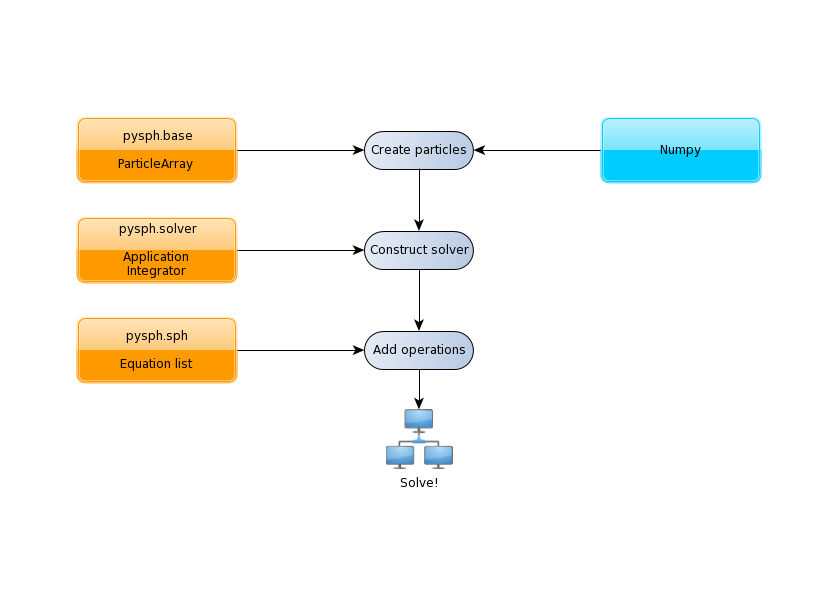
\includegraphics[width = \textwidth]{../pysph-examples-common-steps.png}
\caption{Block Diagram of PySPH}
\end{figure}

The image above is picked from \url{http://pysph.readthedocs.io/en/latest/tutorial/circular_patch_simple.html}\\

The data generated by the simulations can be viewed using the mayavi viewer tool built for PySPH which reads in the numpy files and displays them.

